\section{Auswertung} \label{sec:auswertung}

\subsection{Modell} \label{subsec:modell}

Für die Berechnung der potentiellen Energie benützen wir das Modell Park Avenue 432, eines der höchsten reinen Wohnhochhäusern auf der Welt. Die stolze Höhe und der über das ganze Gebäude gleichbleibende quadratische Grundriss sind ideal für unsere Berechnungen. Für die Wassermengenberechnung stützen wir uns auf die Angaben des durchschnittlichen Wasserverbrauch in Amerika pro Person und Tag: 314\si{L}. \cite{waterUsAmerica}

\begin{figure} [H]
	\centering
	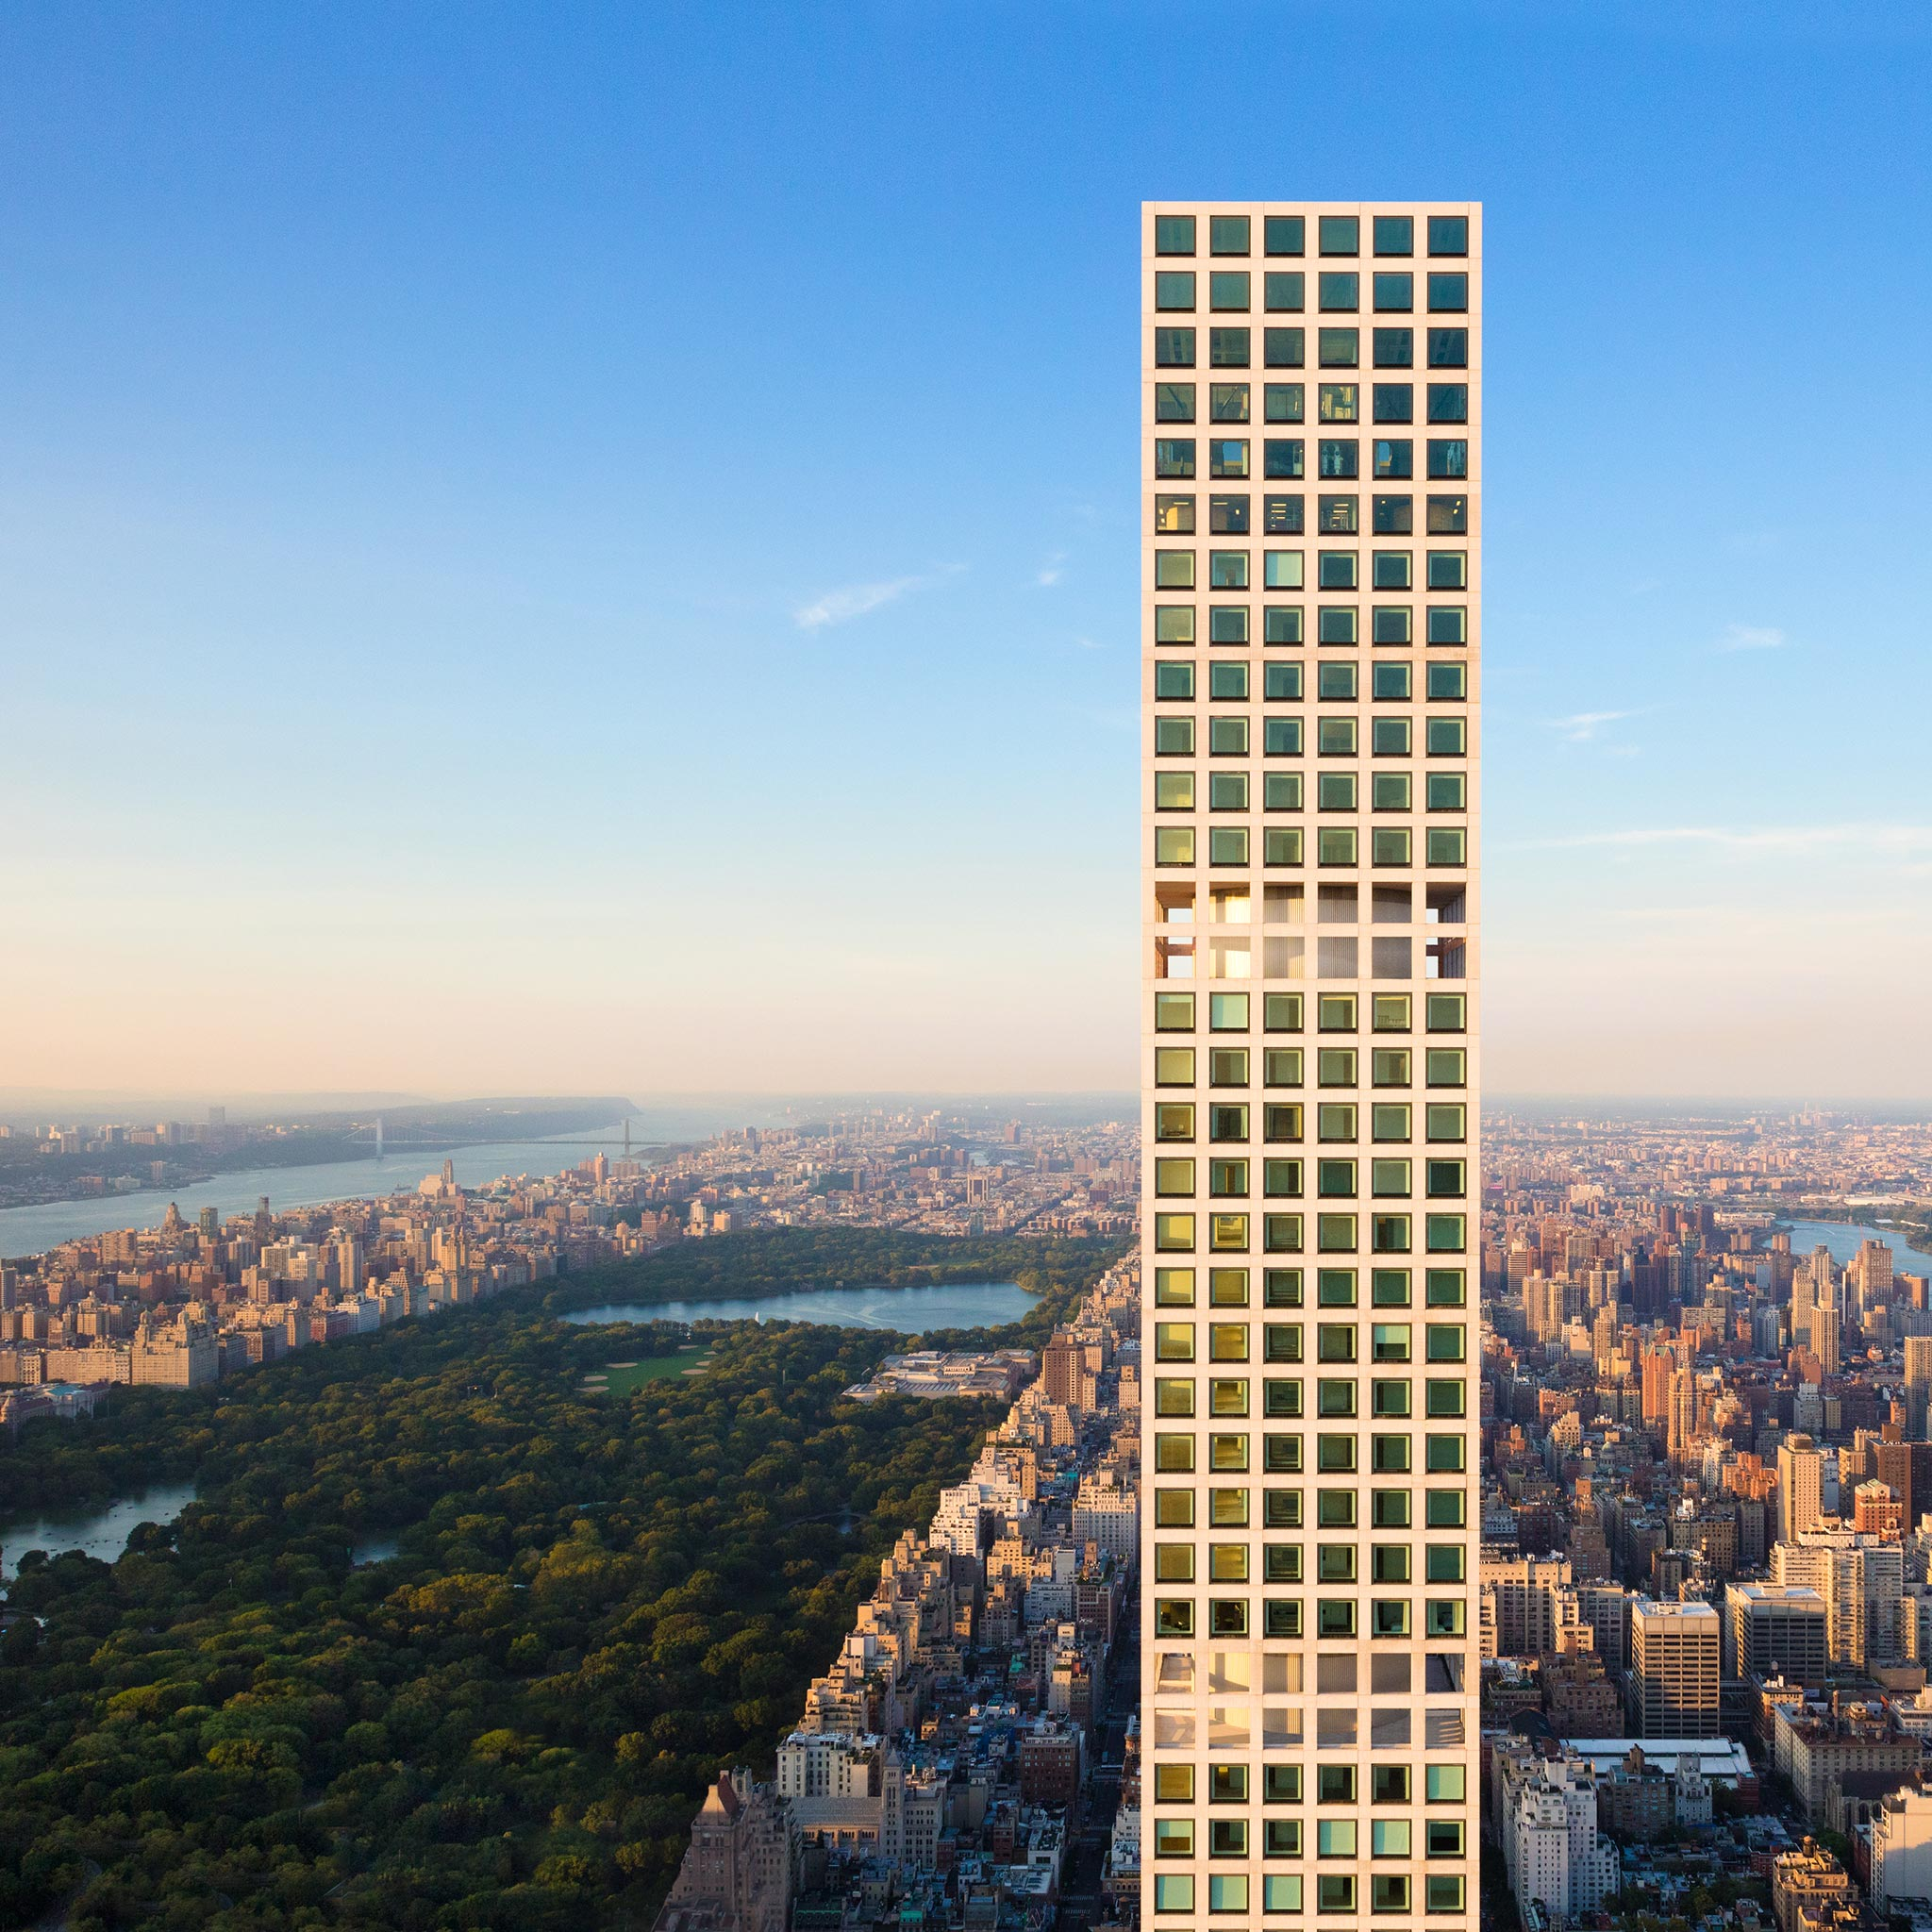
\includegraphics[width=12cm]{parkAvenue.jpg}
	\caption{Park Avenue 432 \cite{432_Park_Avenue}}
	\label{fig:Park_Avenue_432}
\end{figure}

\begin{table}[H]
\centering
\begin{tabular}{ll}
Name:				&Park Avenue 432\\
Höhe: 				&426m\\          
Etagen:				&84 Obergeschosse, 1 Erdgeschosse, 3 Untergeschosse\\
Etagenhöhe:			&4.72m\\
Hoechste Etage:		&392.1m\\
Wohnungen:			&146\\
Speziell:			&alle 12 Etagen 2 Etagen leer\\           
\end{tabular}
\end{table}

\newpage


\subsection{Energieberechnung} \label{subsec:energieberechnung}

Die Endgeschwindigkeit des Wassers kann mit folgender Formel berechnet werden:
\begin{center}
\[
	v = \sqrt{2 \cdot g \cdot h}
\]
\end{center}

Die Einheit der Geschwindigkeit \(v\) ist \si{m/s}, das Schwerefeld \(g\) auf der Erde besitzt den Wert 9.81~\si{N/kg}, und die Höhe \(h\) hat die Einheit \si{m}.

\bigskip

Die Energie, die gewonnen werden kann, wird mit folgender Formel berrechnet:

\begin{center}
\[
	E =\frac 12\ \cdot m \cdot v^2
\]
\end{center}

Die Energie \(E\) hat die Einheit \si{J}, die Einheit der Geschwindigkeit \(v\) ist \si{m/s}, und die Masse \(m\) hat die Einheit \si{kg}

\bigskip

Um die Leistung in \si{kWh} zu erhalten wird forlgende Formel verwendet:

\begin{center}
\[
	P = \frac{E \cdot \eta}{3.6\si{MJ}}
\]
\end{center}

Die Leistung \(P\) hat die Einheit \si{W} und der Wirkungsgrad \(\eta\) besitzt keine Einheit.

\newpage

Mit diesen Mathematischen Grundlagen kann nun die Leistung an unserem Modellhochhaus für die Grobkonzepte berechnet werden. Für die Berchnungen wird angenommen das pro Wohnung 2.5 Personen leben und sie einen Durchschnittverbrauch pro Tag von 314\si{l} haben. Bei 146 Wohnungen und 74 Nutzbaren Etagen leben 5 Personen pro Etage. Es wird somit 1570\si{l} pro Etage pro Tag verbraucht. Im Anhang befindet sich das vereinfachte Modell (\ref{fig:VereinfachtesModel} \nameref{fig:VereinfachtesModel}) des Hochhauses, von der die Berechnungen ausgehen. Das gesamte hochhaus wird zur vereinfachung in 6 Blöcke eingeteilt. Dies ist in der Abbildung \ref{fig:EinteilungBloecke} \nameref{fig:EinteilungBloecke} ersichtlich.

\begin{figure} [H]
	\centering
	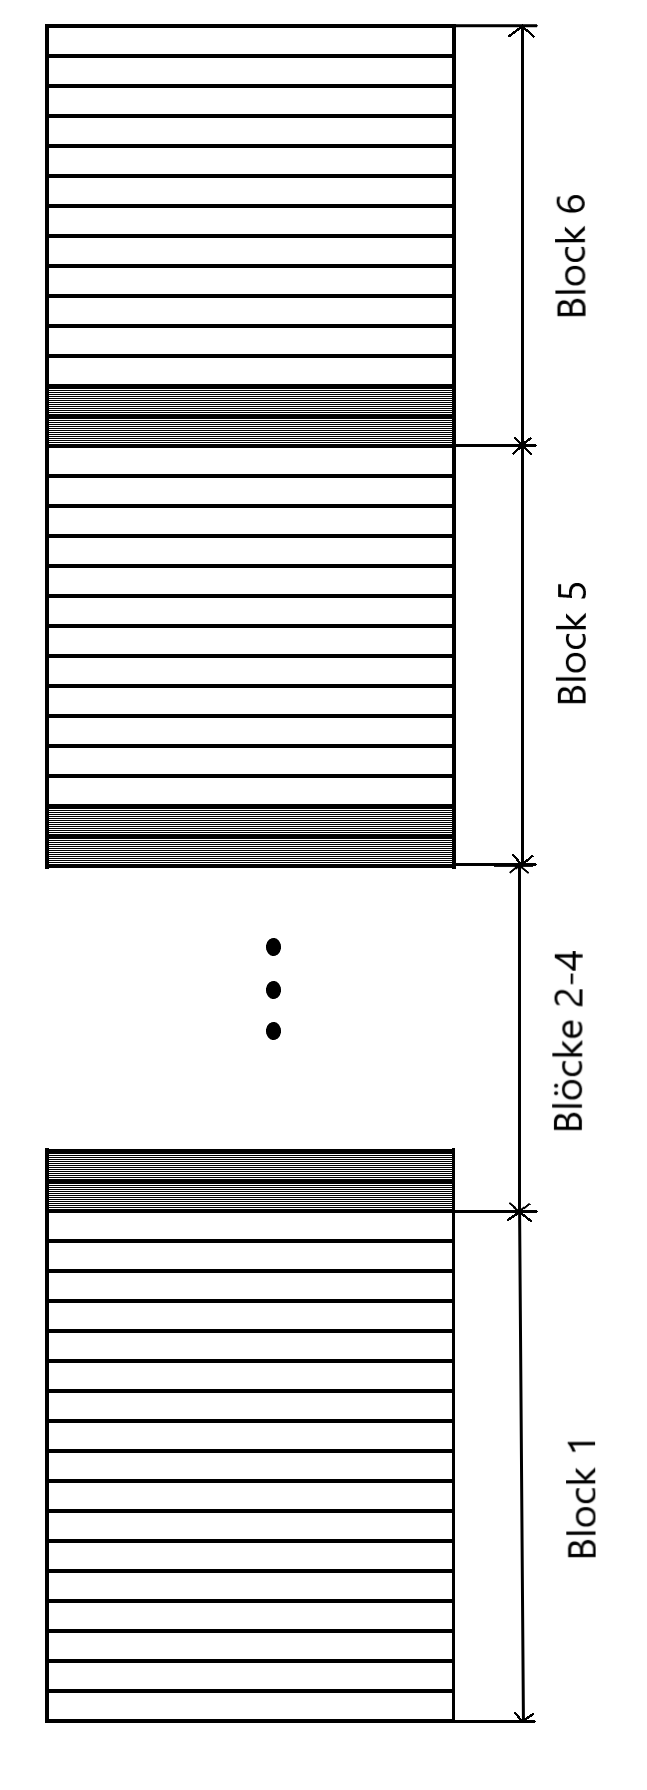
\includegraphics[width=4cm]{EinteilungBloecke.png}
	\caption{Blockeinteilung des Hochhauses}
	\label{fig:EinteilungBloecke}
\end{figure}

\newpage

\paragraph{Grobkonzept 1} 

Im Grobkonzepts 1 wird die Geschwindigkeit des Wassers ausgenutzt. Wie bereits im Recherchedokument (\cite{recherchedokument}) berechnet, wird das Wasser ab ca. 10m nicht mehr merklich schneller. Um möglichst viel Energie zu erzeugen wird in jeder zweiten Etage, bzw all 9.44 \si{m} ein kleines Wasserrad eingebaut. Ingesamt werden 50 Wasserräder eingebaut. Dies ist in der Abbildung \ref{fig:PrinzipGrobkonzept1} \nameref{fig:PrinzipGrobkonzept1} ersichtlich. Die Geschwindigkeit des Wassers beträgt bei einer Höhe von zwei Etagen 8.5\si{m/s} und bei einer Etage 6.5\si{m/s}

\begin{figure} [H]
	\centering
	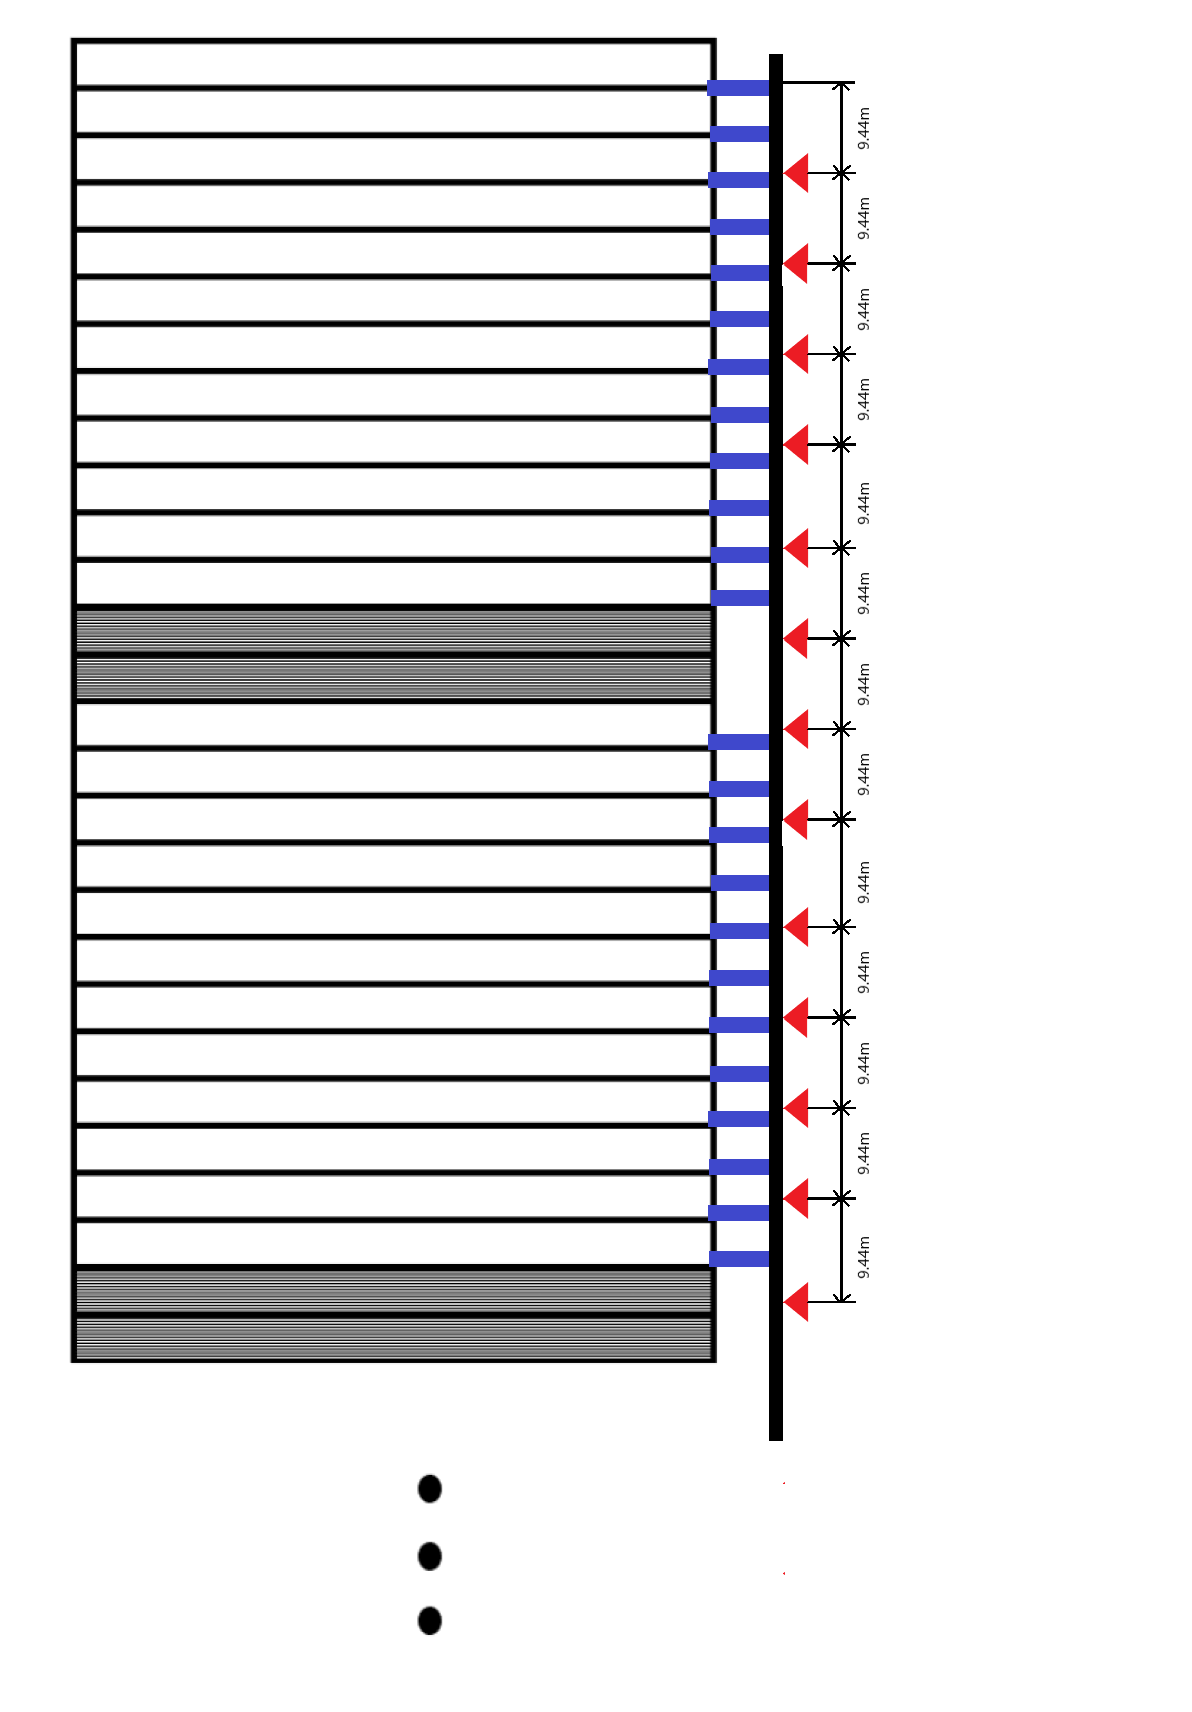
\includegraphics[width=6cm]{PrinzipGrobkonzept1.png}
	\caption{Prinzip Grobkonzep 1}
	\label{fig:PrinzipGrobkonzept1}
\end{figure}

Mit diesem Konzept wird ingesamt 21.5\si{kWh} pro Tag gewonnen, dies entspricht bei Stromkosten von 20\si{rp} einen Wert von 4.30\si{Fr}. Die Leistungsberechnungen sind im Anhang \ref{fig:BerechnungGrobkonzept1} \nameref{fig:BerechnungGrobkonzept1} zu finden.

\newpage

\paragraph{Grobkonzept 2}

Im Grobkonzepts 2 wird die Geschwindigkeit des Wassers ausgenutzt. Um den Luftwiderstand zu eliminieren werden nun Druckleitungen eingebaut die komplett mit Wasser gefüllt sind. So kann eine grössere Geschwindigkeit aufgebaut werden. In den unbenutzen Etagen wird das Wasser gesammelt und mit einer Druckleitung bis zur Turbine ganz unten geführt. Dies ist in der Abbildung \ref{fig:PrinzipGrobkonzept2} \nameref{fig:PrinzipGrobkonzept2} ersichtlich.

\begin{figure} [H]
	\centering
	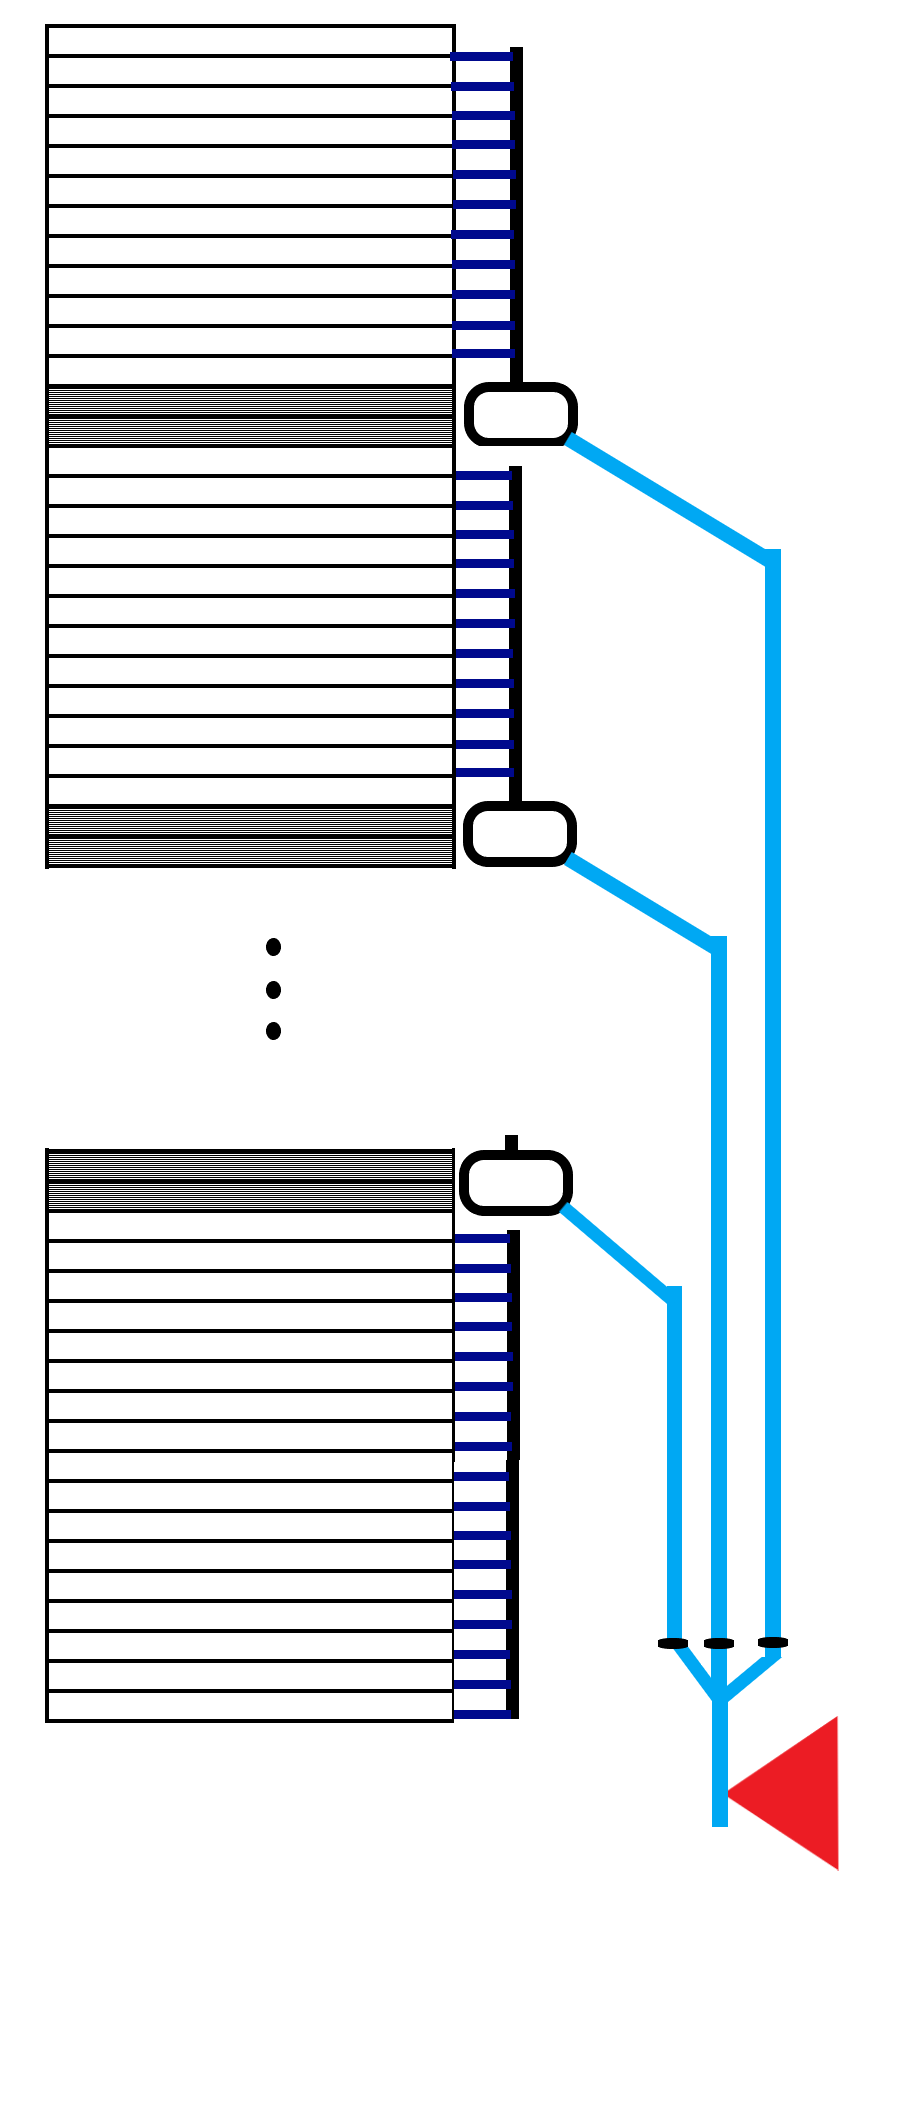
\includegraphics[width=6cm]{PrinzipGrobkonzept2.png}
	\caption{Prinzip Grobkonzep 2}
	\label{fig:PrinzipGrobkonzept2}
\end{figure}

Mit diesem Konzept wird ingesamt 44.59\si{kWh} pro Tag gewonnen, dies entspricht bei Stromkosten von 20\si{rp} einen Wert von 8.92\si{Fr}. Die Leistungsberechnungen sind im Anhang \ref{fig:BerechnungGrobkonzept2} \nameref{fig:BerechnungGrobkonzept2} zu finden.

\newpage

\paragraph{Grobkonzept 3}

Im Grobkonzepts 3 wird die Geschwindigkeit des Wassers ausgenutzt. Um den Luftwiderstand zu eliminieren werden nun Druckleitungen eingebaut die komplett mit Wasser gefüllt sind. So kann eine grössere Geschwindigkeit aufgebaut werden. In den unbenutzen Etagen wird das Wasser gesammelt und mit einer Druckleitung bis zur Turbine vor dem nächsten Tank geführt. Dies ist in der Abbildung \ref{fig:PrinzipGrobkonzept3} \nameref{fig:PrinzipGrobkonzept3} ersichtlich. 

\begin{figure} [H]
	\centering
	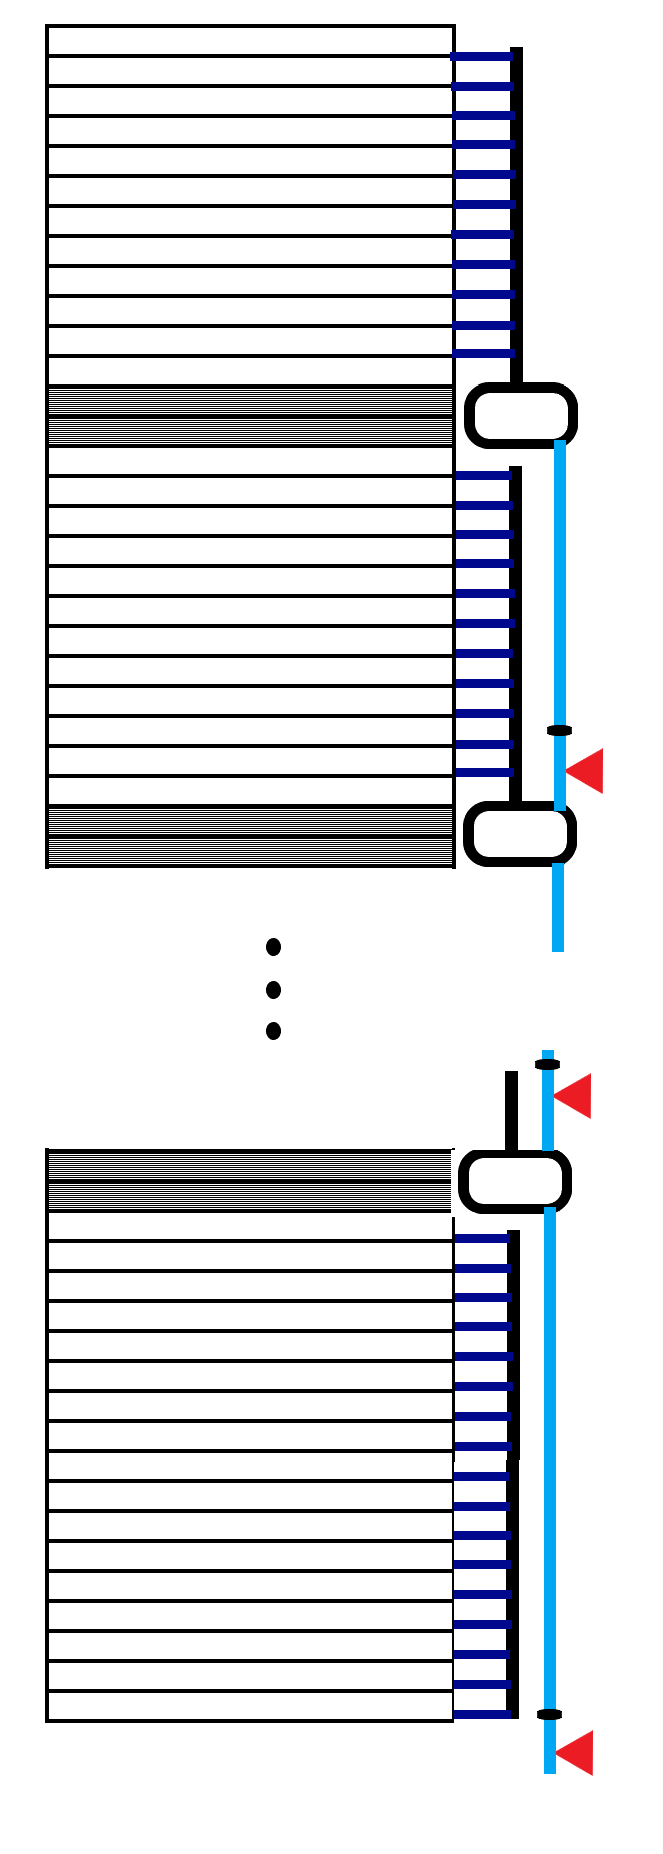
\includegraphics[width=6cm]{PrinzipGrobkonzept3.png}
	\caption{Prinzip Grobkonzep 3}
	\label{fig:PrinzipGrobkonzept3}
\end{figure}

Mit diesem Konzept wird ingesamt 42.62\si{kWh} pro Tag gewonnen, dies entspricht bei Stromkosten von 20\si{rp} einen Wert von 8.53\si{Fr}. Die Leistungsberechnungen sind im Anhang \ref{fig:BerechnungGrobkonzept3} \nameref{fig:BerechnungGrobkonzept3} zu finden.

\newpage

\paragraph{Grobkonzept 4}

Im Grobkonzepts 4 wird die potenzielle Energie des Wassers ausgenutzt. Damit die Wasserlifte nicht zu lang werden, werden diese Blockweise verbaut. Dies ist in der Abbildung \ref{fig:PrinzipGrobkonzept4} \nameref{fig:PrinzipGrobkonzept4} ersichtlich. Die obersten 5 bestehen aus 12 bewohnten und 2 ungenutzten Etagen. Der unterste Block besteht aus 16 bewohnten Etagen. Somit haben 5 Lifte eine Länge von 66.08\si{m} und der unterste Lift eine Länge von 80.24\si{m}

\begin{figure} [H]
	\centering
	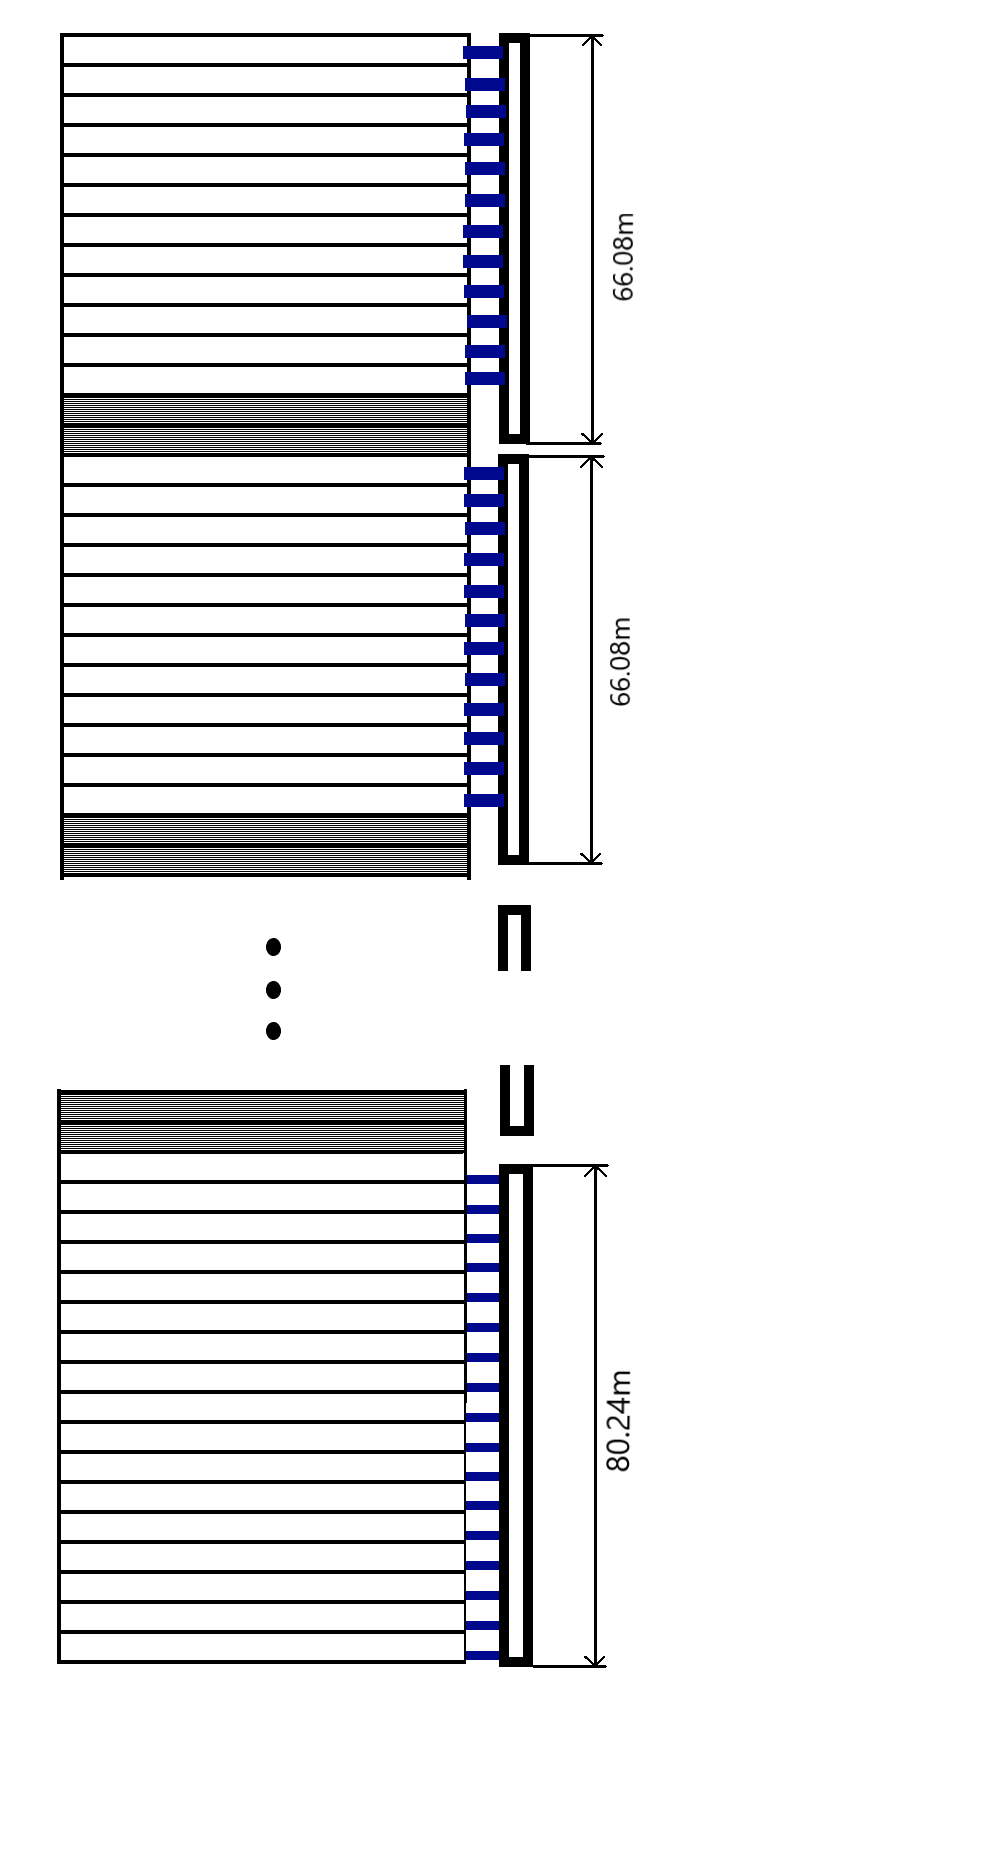
\includegraphics[width=6cm]{PrinzipGrobkonzept4.png}
	\caption{Prinzip Grobkonzep 4}
	\label{fig:PrinzipGrobkonzept4}
\end{figure}

Mit diesem Konzept wird ingesamt 53.08\si{kWh} pro Tag gewonnen, dies entspricht bei Stromkosten von 20\si{rp} einen Wert von 10.62\si{Fr}. Die Leistungsberechnungen sind im Anhang \ref{fig:BerechnungGrobkonzept4} \nameref{fig:BerechnungGrobkonzept4} zu finden.

\newpage